\section{Casos particulares}

\subsection{Caso $R_{3}=0$}

En el caso del \textbf{circuito inversor}, de tomar $R_{3}$ un valor igual a cero, la entrada no inversora quedaría directamente conectada a GND, al igual que la entrada no inversora, de modo que se esperaría que la tensión en la entrada sea nula y por consiguiente no haya tensión a la salida. No obstante, en un $Op$ $Amp$ real sí se mide una pequeña tensión a la salida a pesar de que la tensión de entrada sea cero. Esto último se debe a la presencia de la tensión de offset a la entrada, la cual encuentra su causa en la estructura interna del integrado. Por otro lado, siguiendo exclusivamente la expresión de la ganancia teórica, al ser $R_{3}=0$ se esperaría que la ganancia disminuya. 

En cuanto al \textbf{circuito no inversor}, la eliminación de $R_{3}$ produciría un aumento en la ganancia, al tener la expresión de la ganancia un denominador menor. Asimismo, la expresión de la impedancia de entrada dependería únicamente de la resistencia $R_{4}$ a la entrada. 

\subsection{Caso $R_{4}=0$ en circuito inversor}

La resistencia $R_{4}$ no está presente en las expresiones de la ganancia o la impedancia de entrada, por lo que no se esperarían cambios en sus valores. No se logró identificar su acción sobre algún otro efecto o parámetro del circuito.  

\subsection{$V_{in}$ onda cuadrada de alta frecuencia}

Se propuso pensar en la conveniencia de utilizar un amplificador operacional del LM324 en un circuito con una señal de excitación cuadrada de $1V_{pp}$ con frecuencia entre los $0,3MHz$ y $2MHz$, con $duty$ variante entre 20\% y 80\%. 

Teniendo en cuenta el análisis y las consideraciones hechas a lo largo de este informa, la señal de salida del circuito se vería muy afectada por los distintos fenómenos del operacional y por sus propias limitaciones. Por un lado, teniendo en cuenta que la GBW del operacional a lazo abierto es de $1MHz$, a frecuencias tal altas como $2MHz$ se esperaría que la ganancia sea muy pequeña, por lo que la señal de salida se vería atenuada. Por otra parte, el slew rate afectaría la señal de salida considerando que se estaría trabajando con frecuencias altas y una tensión pico a pico también alta, teniendo en cuenta lo visto anteriormente. 

Para visualizar los efectos, se empleó el caso 1 del circuito no inversor inyectando una señales cuadradas de $1V_{pp}$ con un duty de 50\% a distintas frecuencias.


\begin{figure}[H]
	\centering
	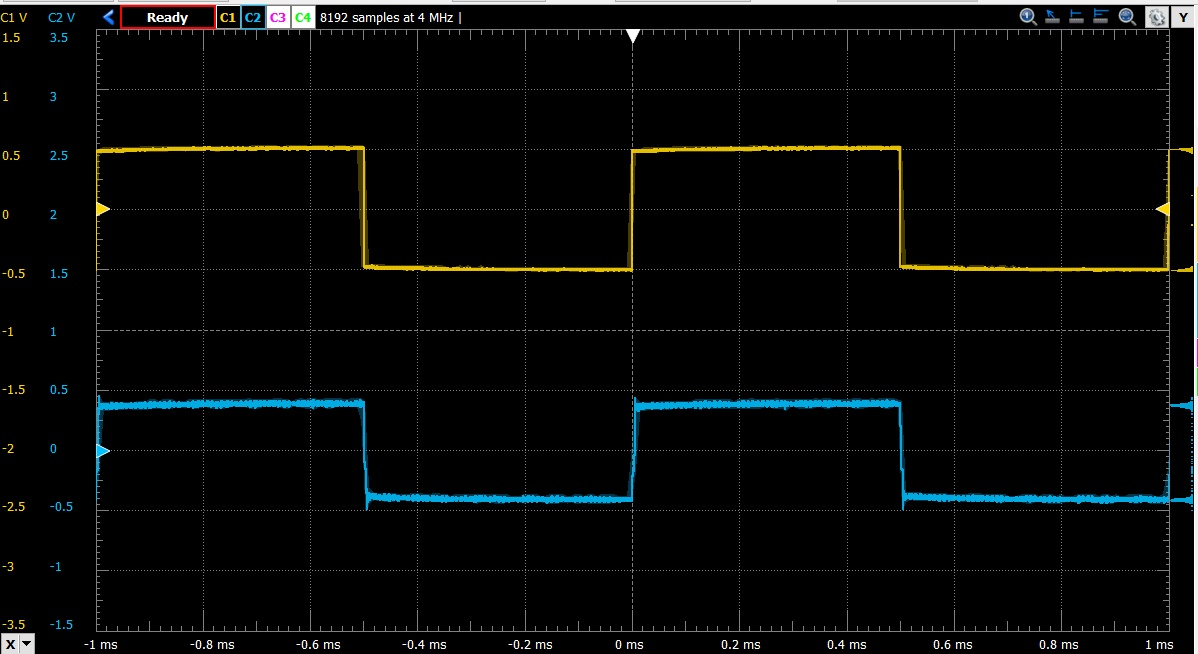
\includegraphics[scale=0.25]{./Imagenes/Sqr1k.jpg}
	\caption{Circuito no inversor caso 1. Señal cuadrada de $1V_{pp}$ a $1kHz$.}
	\label{fig:1kHz}
\end{figure}


\begin{figure}[H]
	\centering
	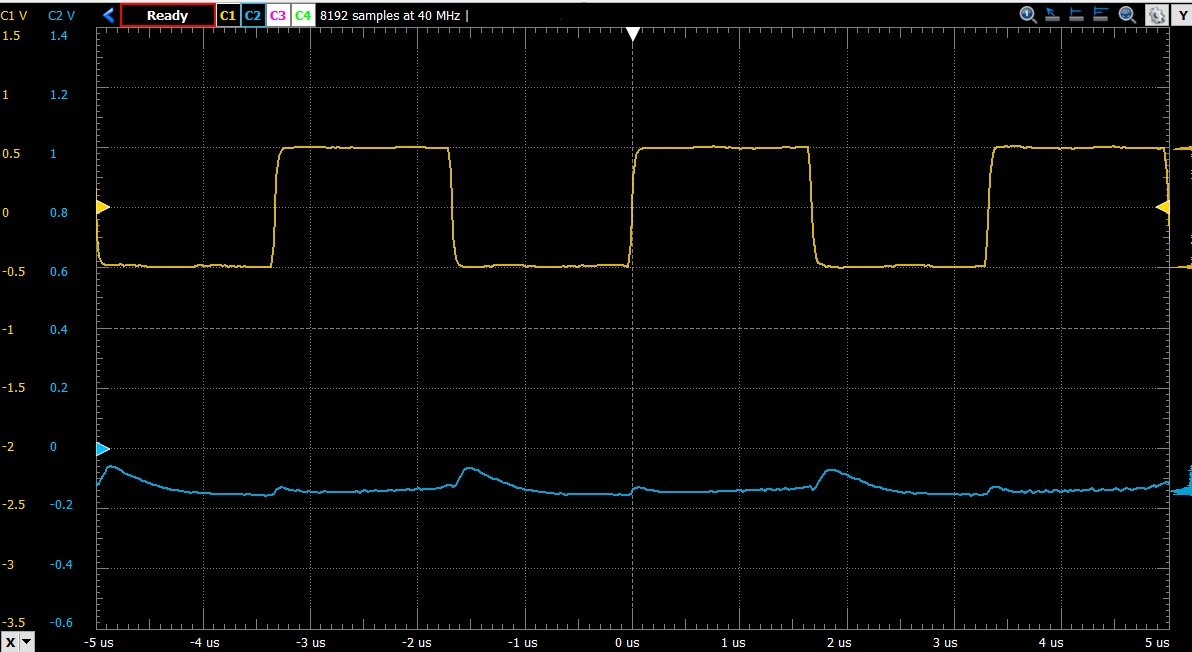
\includegraphics[scale=0.25]{./Imagenes/Sqr300k.jpg}
	\caption{Circuito no inversor caso 1. Señal cuadrada de $1V_{pp}$ a $300kHz$.}
	\label{fig:300kHz}
\end{figure}


\begin{figure}[H]
	\centering
	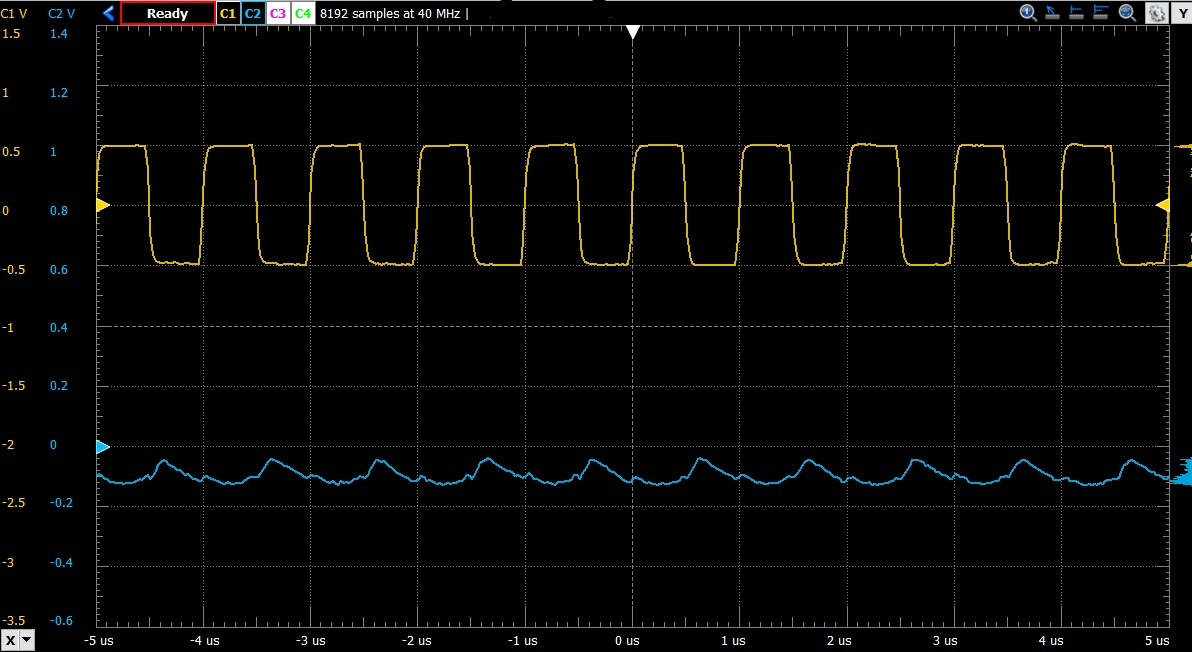
\includegraphics[scale=0.25]{./Imagenes/Sqr1MHz.jpg}
	\caption{Circuito no inversor caso 1. Señal cuadrada de $1V_{pp}$ a $1MHz$.}
	\label{fig:1MHz}
\end{figure}

\begin{figure}[H]
	\centering
	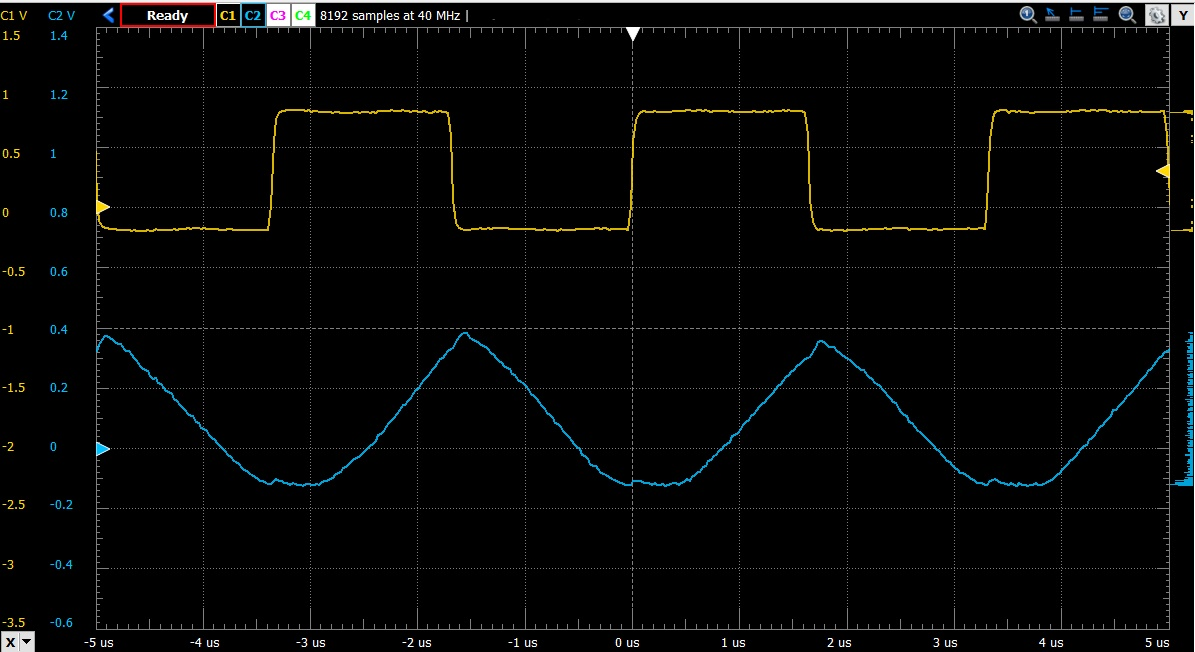
\includegraphics[scale=0.25]{./Imagenes/Sqr1MHzOffset.jpg}
	\caption{Circuito no inversor caso 1. Señal cuadrada de $1V_{pp}$ a $1MHz$ y $0,3V$ de offset.}
	\label{fig:1MHzoffset}
\end{figure}


En la Figura \ref{fig:1kHz} se observa que a una frecuencia de $1kHz$ la señal de salida no sufre prácticamente ninguna distorsión. A frecuencias mas altas, en cambio, la señal de salida resulta sumamente afectada por las limitaciones del operacional. Ejemplos de ello son las Figuras \ref{fig:300kHz} y \ref{fig:1MHz}, a frecuencias de $300kHz$ y $1MHz$ respectivamente. No obstante, de inyectar la misma señal a $1MHz$ con un offset de $0,3V$ la señal de salida muestra una amplificación mucho mayor. 